\chapter{Cliques, Independent sets, Dominating Sets  and Vertex covering }
Rishnak was getting anxious to meet Ajur and discuss other interesting problems with Ajur. Finally Rishnak spotted Ajur and Jura walking along a pond. Rishnak asked Ajur whether there were cliques in his school. This brought in a pet peeve of Ajur. Ajur always felt that the school he was going to had distinct groups. So Ajur had no trouble telling Rishnak that there were distinct cliques in his high school. Rishnak told Ajur that a clique is also a graph theoretic term. A clique is a subgraph of a graph which is complete. Rishnak added that normally we only consider maximal complete subgraphs as cliques. Rishnak added that a maximal complete subgraph of $G$, $H$, means that there is no complete subgraph of $G$ that contains $H$ as a subgraph,

Rishnak drew the following graph in Figure \ref{13g1} and asked Ajur to list the cliques(maximal complete subgraphs).
\begin{figure}
\begin{center}
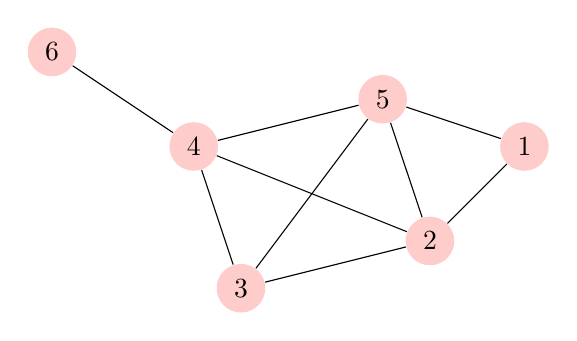
\begin{tikzpicture}
  [scale=.6,auto=left,every node/.style={circle,fill=red!20}]
  \node (n6) at (1,10) {6};
  \node (n4) at (4,8)  {4};
  \node (n5) at (8,9)  {5};
  \node (n1) at (11,8) {1};
  \node (n2) at (9,6)  {2};
  \node (n3) at (5,5)  {3};

  \foreach \from/\to in {n6/n4,n4/n5,n5/n1,n1/n2,n2/n5,n2/n3,n3/n4,n4/n2,n3/n5}
    \draw (\from) -- (\to);

\end{tikzpicture}
\caption{ What are the maximal cliques (complete subgraphs) in this graph}\label{13g1}
\end{center}
\end{figure}

Ajur was tentative in his answer - as he is struggling with all the definitions. Ajur said the three maximal cliques are: 
\begin{enumerate}
    \item Induced subgraph containing vertices 4 and 6.
    \item Induced subgraph containing the vertices 2,3 4 and 5
    \item Induced subgraph containing the vertices 1, 2 and 5
\end{enumerate} 

Rishnak was happy that Ajur understood the definition of maximal cliques. Still he wanted Ajur to find about maximal cliques on another graph shown in Figure \ref{13g21}.
\begin{figure}
\begin{center}
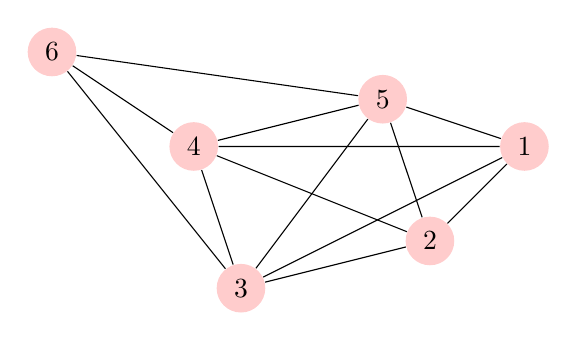
\begin{tikzpicture}
  [scale=.6,auto=left,every node/.style={circle,fill=red!20}]
  \node (n6) at (1,10) {6};
  \node (n4) at (4,8)  {4};
  \node (n5) at (8,9)  {5};
  \node (n1) at (11,8) {1};
  \node (n2) at (9,6)  {2};
  \node (n3) at (5,5)  {3};

  \foreach \from/\to in {n6/n4,n4/n5,n5/n1,n1/n2,n2/n5,n2/n3,n3/n4,n4/n2,n3/n5,n1/n4,n1/n3,n3/n6,n5/n6}
    \draw (\from) -- (\to);

\end{tikzpicture}
\caption{ What are the maximal cliques (complete subgraphs) in this graph}\label{13g21}
\end{center}
\end{figure}

Ajur stared at the figure \ref{13g21} for a few seconds before he answered giving two maximal cliques. He listed them as: 
\begin{enumerate}
    \item Induced subgraph containing vertices 3, 4, 5 and 6.
    \item Induced subgraph containing the vertices 1, 2,3 4 and 5.
\end{enumerate} 
Ajur was frustrated as he was getting some vague definitions and examples. Rishnak admitted that it was his mistake. Graphs are usually used as models for physical or social processes. For example, when we consider the cliques in a school, you can model the students as vertices and two students belong to the same group as an edge between the associated vertices\footnote{We have a binary relation here.}. Clusters in data science are closely related to cliques. Since graphs are models of social a

Rishnak wanted Ajur to know about Independent set in a graph, An independent set in a graph is a set of vertices that are mutually nonadjacent i.e., a subset of vertices that does not include any adjacent vertices. Ajur immediately said that Independent set and Clique seem to be related. Rishnak could not control his smile. Rishnak remembered that he had not told Ajur about complement of a graph. A complement of a graph $G=(V,E)$ is another graph $H=(V,E_1)$. Both of them have the same vertex set. But if two vertices are adjacent in G, they are not adjacent in H and if two vertices are not adjacent in G, then they are adjacent in H. Ajur drew the complement of the graph shown in Figure \ref{13g1} as shown in Figure \ref{13g21}

\begin{figure}
\begin{center}
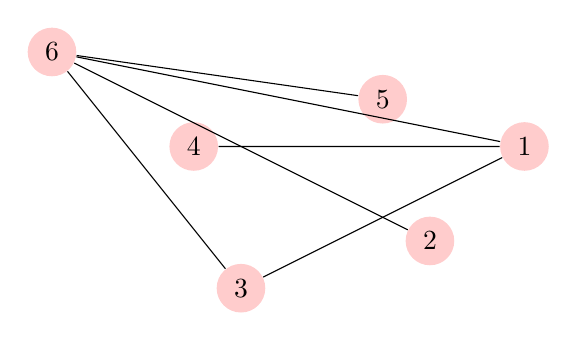
\begin{tikzpicture}
  [scale=.6,auto=left,every node/.style={circle,fill=red!20}]
  \node (n6) at (1,10) {6};
  \node (n4) at (4,8)  {4};
  \node (n5) at (8,9)  {5};
  \node (n1) at (11,8) {1};
  \node (n2) at (9,6)  {2};
  \node (n3) at (5,5)  {3};

  \foreach \from/\to in {n6/n5,n6/n3,n6/n2,n6/n1, n1/n3,n1/n4}
    \draw (\from) -- (\to);

\end{tikzpicture}
\caption{ Complement of Graph in \label{13g1}}\label{13g2}
\end{center}
\end{figure}

Ajur further said that the number of edges in the complement of the graph will be $n\times\frac{n-1}{2}-e$ where original graph has $n$ vertices and $e$ edges. Hence a maximal clique in a graph will be an independence set in the complement of the graph. For the graph shown in Figure \ref{13g2}, the maximal independence sets are $\{2,3,4,5\}, \{1,2,5\} , \{4,6\}$. These are also the maximal cliques in Figure \ref{13g1}. In a bipartite graph shown below \ref{13g3}, the independent sets are $\{1,2\}, \{3,4,5,6\}, \{2,6\}$.
\begin{figure}
\begin{center}
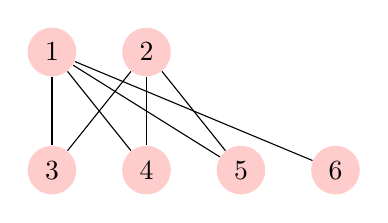
\begin{tikzpicture}
  [scale=.3,auto=left,every node/.style={circle,fill=red!20}]
  \node (n1) at (1,7) {1};
  \node (n2) at (5,7)  {2};
  \node (n3) at (1,2)  {3};
  \node (n4) at (5,2) {4};
  \node (n5) at (9,2)  {5};
   \node (n6) at (13,2) {6};
  
   \foreach \from/\to in {n1/n3,n1/n4,n1/n5,n2/n3,n2/n4,n2/n5,n1/n6}
    \draw (\from) -- (\to);
    \end{tikzpicture}
\caption{ A Bipartite Graph with 6 vertices and 7 edges}\label{13g3}
\end{center}
\end{figure}
